\section{Porovnanie $PCGS$ s $g$-systémami}

\begin{veta}
Pre každý $PCGS_mREG$ $\Gamma$ existuje $g$-systém $G$ taký, že
$L(G)=L(\Gamma)$
\end{veta}

\begin{dokaz}
Nech $\Gamma=(N,K,T,G_1,\dots ,G_m)\in PCGS_mREG$. Chceme
zostrojiť $g$-systém $G=(N',T,M,\sigma)$ taký, že $L(G)=L(\Gamma)$
\\ Najskôr, ako sme to už urobili v niektorých predchádzajúcich
dôkazoch tejto kapitoly, si všimneme štruktúru slova, ktoré máme
vyrobiť. Slovo $w\in L(\Gamma)$ pozostáva z podslov, ktoré boli
generované jednotlivými gramatikami $\Gamma$. Keďže neuvažujeme
nejaký špeciálny typ komunikačnej štruktúry, nemôžeme o
postupnosti podslov prislúchajúcich k jednotlivým gramatikám
vysloviť žiaden predpoklad okrem toho, že zrejme prvé podslovo
bude generované gramatikou $G_1$.
\\ Simuláciu $\Gamma$ $g$-systémom $G$ môžeme rozdeliť do
niekoľkých fáz:
\begin{description}
  \item[Inicializácia] (obr.\ref{pcgsgs1})

\begin{figure}[ht]
  \centering
  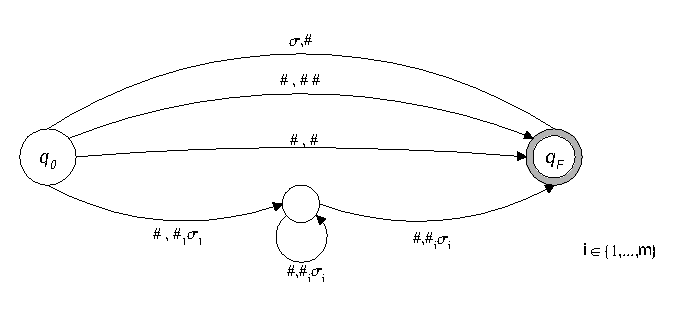
\includegraphics{img/pcgs/pcgsgs1}
  \caption{Časť 1-a-prekladača pre fázu inicializácie}\label{pcgsgs1}
\end{figure}

  Najskôr $G$ uhádne počet komunikácií uskutočnených pri
  generovaní slova $w$ t.j. z koľkých podslov pozostáva $w$. Toto
  bude $G$ simulovať tak, že vygeneruje príslušný počet neterminálov $\#$.
  Potom $G$ uhádne príslušnosť jednotlivých podslov ku gramatikám
  t.j. ktoré podslovo bolo vyrobené ktorou gramatikou. Podľa toho
  bude $G$ prepisovať $\#$ na $\#_i\sigma_i$ (akési zárodky budúcich podslov),
  teda takto reprezentované podslovo bolo v $\Gamma$ generované gramatikou
  $G_i$. Zrejme prvý neterminál $\#$ bude prepísaný na $\#_1\sigma_1$, keďže
  prvé podslovo vygenerovala $G_1$

  \item[Prepisovací krok] (obr.\ref{pcgsgs2})
\begin{figure}[ht]
  \centering
  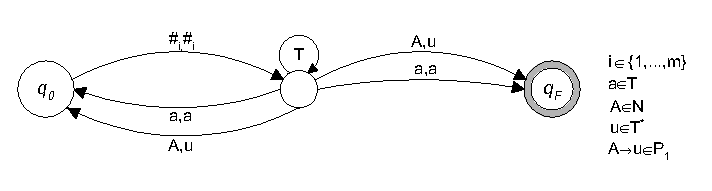
\includegraphics{img/pcgs/pcgsgs2}
  \caption{Časť 1-a-prekladača pre fázu prepisovania}\label{pcgsgs2}
\end{figure}

  $g$-systémy vedia veľmi jednoducho simulovať regulárne
  gramatiky. V príslušnej vetnej forme skopírujú všetky
  neterminály a neterminál prepíšu podľa pravidiel regulárnej
  gramatiky. Náš $g$-systém $G$ bude vedieť simulovať všetky gramatiky
  $\Gamma$, pričom keď pri prechádzaní vetnej formy narazí na
  neterminál $\#_i$, bude simulovať gramatiku $G_i$ t.j. terminály
  sa skopírujú a neterminál sa prepíše podľa pravidiel v $G_i$.
  Môže sa stať, že vetná forma $G_i$ nebude obsahovať neterminál,
  preto musíme do $G$ pridať zopár šípok naviac, ktoré uhádnu, že
  nejaký terminál je vo vetnej forme danej gramatiky $G_i$
  posledný, aby sa nám nestalo, že v nejakom stave bude $G$
  na vstupe očakávať neterminál z $G_i$, ale dostane $\#_j$

  \item[Komunikačný krok] (obr.\ref{pcgsgs3})
\begin{figure}[ht]
  \centering
  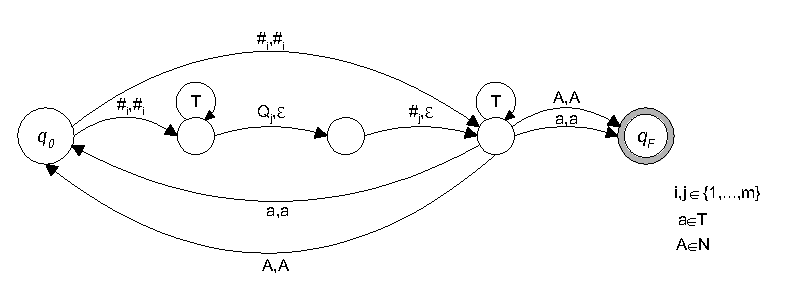
\includegraphics{img/pcgs/pcgsgs3}
  \caption{Časť 1-a-prekladača pre fázu komunikácie}\label{pcgsgs3}
\end{figure}

  $G$ sa, predtým ako začne čítať vstup, niekedy rozhodne, že
  vo vetnej forme sa nachádzajú nejaké komunikačné symboly, teda
  má nastať komunikačný a nie prepisovací krok. $G$ uhádne podslovo,
  v ktorom sa nachádza komunikačný symbol $Q_j$ pre nejaké $j\in\{ 1\dots
  m\}$. Nech je toto podslovo generované gramatikou $G_k$. To znamená,
  že keď $G$ má na vstupe $\#_i$, môže sa
  rozhodnúť, či toto podslovo obsahuje alebo neobsahuje $Q_j$. Ak
  sa rozhodne, že nie, všetky terminály a prípadný neterminál
  skopíruje. Ak sa rozhodne, že áno, kopíruje terminály a očakáva
  $Q_j$. Ak sa objaví nejaký iný neterminál, znamená to, že $G$
  hádal nesprávne a zasekne sa. Ak na vstup príde $Q_j$, tak ho
  $G$ vymaže a očakáva symbol $\#_j$, ktorý tiež vymaže a zvyšok podslova
  skopíruje. Ak sa vo vetnej forme vyskytnú vedľa seba symboly
  $Q_j,\#_j$ znamená to, že v inicializácii $G$ správne uhádol
  následnosť týchto dvoch podslov t.j. uhádol, že gramatika $G_k$
  si vyžiada vetnú formu generovanú gramatikou $G_j$. Ak sa vo vetnej
  forme vyskytne dvojica $Q_j\#_i$ pre $j\neq i$, tak $G$ v inicializácii hádal
  zlú následnosť podslov a zasekne sa. Treba si uvedomiť, že toto
  naozaj simuluje komunikáciu, lebo v ďalšom prechode tým, že sme vymazali
  $Q_j\#_j$, bude podslovo pôvodne generované $G_j$ už súčasťou
  podslova generovaného $G_k$, a teda aj prepísanie prípadného
  neterminálu druhého podslova bude podliehať simulácii pravidiel
  $G_k$
  \item[Overovanie]
   V doterajšej simulácii sme ešte neuvažovali situáciu, že dve rôzne
  gramatiky $G_k,G_l$ $k\neq l$ naraz v tom istom kroku vygenerujú
  $Q_j$ pre nejaké $j\in \{ 1\dots m\}$. V $\Gamma$ to znamená, že
  vo vetnej forme oboch gramatík sa objaví ten istý obsah vetnej
  formy gramatiky $G_j$. V doteraz uvažovanej simulácii máme
  zabezpečené, že $G$ v inicializácii dobre uhádne dvojice
  $\#_k\sigma_k\#_j\sigma_j$ a $\#_l\sigma_l\#_j\sigma_j$, ale
  nemáme nijako zabezpečené, že simulácie odvodení gramatiky $G_j$
  budú na dvoch miestach rovnaké. Preto komunikačný krok upravíme
  nasledovne. $G$ si bude počas komunikačného kroku v stave pamätať
  $query$, ktoré už úspešne odstránil, a ak nájde vo vetnej forme
  ďalší taký symbol, zasekne sa. Tým sme zabezpečili,
  že komunikačný krok sa vykonaná len vtedy, keď vo vetnej forme
  nie sú viacnásobné $query$.
  \\ Keď sa $G$ rozhodne, že vo vetnej forme je viacnásobný
  $query$, tak uhádne a v stave si zapamätá $Q_j$, ktorý je
  viacnásobný a na začiatok vetnej formy dá špeciálny znak, upozorňujúci,
  že táto vetná forma je v stave overovania. Potom prehľadáva
  (kopíruje symboly) vetnú formu, a keď nájde prvý $Q_j$, tak ho
  vymaže, očakáva $\#_j$ ten tiež vymaže, v stave si zapamätá
  nasledujúci symbol podslova (pôvodne začínajúceho $\#_j$) a za
  tento symbol umiestni opäť špeciálny symbol $\pounds$ ukazujúci pokiaľ
  prečítal prvé overované podslovo. Zvyšok podslova skopíruje a v
  ďalších podslovách hľadá $Q_j$. Ak v podslove $Q_j$ nenájde, tak
  ho celé skopíruje, inak ho opäť vymaže spolu s očakávaným $\#_j$
  a porovnáva nasledujúci symbol podslova s tým, ktoré si
  zapamätal. Ak sa zhodujú, za tento symbol umiestni špeciálny
  znak $\$$ ukazujúci pokiaľ už podslovo overil a zvyšok podslova
  skopíruje, inak sa zasekne. Takto $G$ prejde celú vetnú formu.
  \\ Pri ďalšom prechode je na začiatku vstupu špeciálny symbol,
  ktorý hovorí, že máme pokračovať v overovaní. $G$ kopíruje
  symboly, až kým nenájde $\pounds$. Ten vymaže, zapamätá si ďalší
  symbol z overovaného podslova a zaň umiestni $\pounds$, zvyšok
  podslova skopíruje. V ďalších podslovách hľadá $\$$, a keď ho
  nájde, vymaže ho, skontroluje nasledujúci symbol so zapamätaným
  (ak sa nezhoduje, zasekne sa) a zapíše $\$$. Takýmto spôsobom
  dokáže $G$ overiť zhodnosť podslov, ktoré si dve gramatiky
  presunú do svojej vetnej formy, keď naraz vygenerujú rovnaké
  $query$.
  \\ $G$ sa niekedy na začiatku ďalšieho prechodu môže rozhodnúť,
  že už je overené celé podslovo t.j. za symbolmi $\pounds$, $\$$
  je nejaký $\#_i$. Vtedy $G$ vymaže špeciálny symbol na začiatku
  a symboly $\pounds$, $\$$ vo vetnej formy pričom overuje, či za
  týmito symbolmi sú naozaj nejaké $\#_i$, inak sa zasekne

  \item[Ukončenie] (obr.\ref{pcgsgs4})

\begin{figure}[ht]
  \centering
  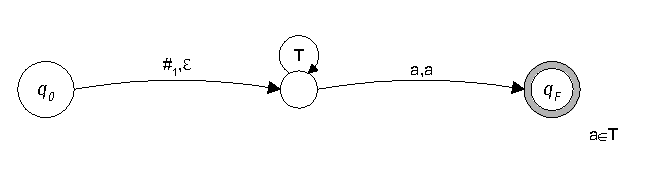
\includegraphics{img/pcgs/pcgsgs4}
  \caption{Časť 1-a-prekladača pre fázu ukončenia}\label{pcgsgs4}
\end{figure}

  $G$ sa v počiatočnom stave niekedy rozhodne, že vetná forma
  obsahuje symbol $\#_1$ na začiatku a potom už len terminály. To znamená,
  že už nebudú nasledovať ani prepisovacie ani komunikačné kroky, teda simulácia
  $\Gamma$ už skončila. V tomto kroku stačí odstrániť symbol
  $\#_1$, čím dostaneme terminálne slovo
\end{description}
Čitateľ si určite všimol, že najzložitejšia z fáz bolo
overovanie\footnote{preto sme ani neuviedli príslušný obrázok
1-a-prekladača, ktorý by bol značne neprehľadný}. Skúsme sa preto
zamyslieť, čo by sa stalo, keby sme overovanie zo simulácie
vynechali. V takomto prípade sa však musíme obmedziť na
simulovanie $PCGS$ s komunikačnou štruktúrou, ktorá nedovoľuje,
aby v orientovanom grafe reprezentujúcom túto štruktúru existovali
dve rôzne hrany vedúce do jedného vrchola. To napríklad spĺňajú
štruktúry one-way array, one-way ring, tree, centr. Ak $\Gamma$ s
takouto komunikačnou štruktúrou vygeneruje slovo v čase $T(n)$,
tak $G$ vygeneruje toto slovo v rovnakom čase, teda $g$-systém
zachováva časovú zložitosť $PCGS$.
\\ Ak sa vrátime späť k všeobecnej komunikačnej štruktúre,
overovanie zhorší časovú zložitosť polynomiálne
\end{dokaz}
